\documentclass[12pt,a4paper,twoside,%
BCOR12mm,DIV12,%
headsepline,%
cleardoubleempty,chapterprefix,parskip,%
liststotoc,idxtotoc,bibtotoc]{scrbook}

\usepackage[english, ngerman]{babel}
\usepackage[utf8]{inputenc}
\usepackage[T1]{fontenc}
\usepackage{mathptmx}
\usepackage[scaled=0.92]{helvet}
\usepackage{courier}
\usepackage{amsmath}
\makeatletter
\def\displaymath{\typeout{*** Do not use DISPLAYMATH. Use \[...\] instead ***}}
\def\eqnarray{\typeout{*** Do not use EQNARRAY(*). Use align(*)-environment instead ***}}
\makeatother
\usepackage{amsfonts}
\usepackage{amstext}
\usepackage{subfigure}
\usepackage{color}
\usepackage{wrapfig}	% let text float around pictures
\usepackage{graphicx}
\usepackage{ifpdf}
\usepackage{makeidx}
\usepackage{nomencl}
\usepackage{setspace}

\usepackage{listings}

% first include hyperref, then cite
\usepackage[plainpages=false,pdfpagelabels]{hyperref}
\usepackage{cite}

\usepackage{lscape}
\usepackage{tabularx}

\ifpdf
    \definecolor{brown}{cmyk}{0, 0.81, 1, 0.60}
    \hypersetup{%
      pdftitle={Verteiltes Veranstaltungsmanagement mit einer mobilen Webanwendung}, %%%% HIER AENDERN!!!
      pdfsubject={Bachelorarbeit},
      pdfauthor={Christian Meter},           %%%% HIER AENDERN!!!
      pdfkeywords={KEYWORDS},      %%%% HIER AENDERN!!!
      colorlinks=false, urlcolor=blue, citecolor=brown,
      bookmarksnumbered=true,
    }
\else   
\fi

\listfiles

\begin{document}
\onehalfspacing

\frontmatter

\pdfbookmark[0]{Titelseite}{tit}
% Titelseite

\begin{titlepage}
  \centering
  
\includegraphics[width=5cm]{fig/unilogo}\\

  \vfill
  \huge
  Installations- und Bedienungsanleitung\\für die Meißner Webanwendung\\*[40pt]
  \normalsize

  \vfill
  \large
  \normalsize
  von\\
  \Large
  Christian Meter\\

  \vspace{5mm}
  \normalsize
  aus\\ Remscheid\\[1cm]
  vorgelegt am\\[5mm]
  Lehrstuhl für Rechnernetze und Kommunikationssysteme\\
  Prof.\ Dr.\ Martin Mauve\\ 
  Heinrich-Heine-Universität Düsseldorf\\[0.5cm]
  September 2013\\[0.5cm]
  Betreuer:\\
  %Dipl.\ Wirtsch.-Inf.\ Vorname Nachname\\
  Philipp Hagemeister M.\,Sc.
    
\end{titlepage}


%%% Local Variables: 
%%% mode: latex
%%% TeX-master: "master"
%%% End: 


\cleardoublepage

\pdfbookmark[0]{Abstract}{abstract}
\begin{center} 
\huge Abstract
\end{center}

Hier beschreibe ich nun auf einer Seite, welches Problem ich betrachtet, wie ich es gelöst habe
und was die Hauptergebnisse meiner Arbeit sind.

Entwicklung einer Webanwendung, die das Verwalten von Veranstaltungen mit vielen Benutzern und Helfern ermöglicht. Touchoptimierte Seiten für mobile Endgeräte ermöglichen eine einfache Handhabung und bieten den gleichen Funktionsumfang wie die Desktopanwendung.\par

Die Meißner App ist für die Nutzung im Außenbereich auf einer großen Fläche gedacht, weshalb über eine Echtzeitaktualisierung mit WebSockets den Austausch der Geolocations einzelner Endgeräte ermöglicht wird. Dadurch können die Standorte der Helfer erfragt werden und diese dann effektiver durch Wegoptimierung eingesetzt werden.\par

Eigene Module für PUSH-Benachrichtigungen und der Möglichkeit einzelne Veranstaltungen zu abonnieren wurden implementiert. 

Kurze Zusammenfassung (ca. 200 Wörter)\\
* Klar und prägnant: Worum gehts? Was wurde herausgefunden? Warum ist das wichtig?\\
* Aushängeschild des Artikels; Reviewer bilden sich eine Meinung, Leser entscheiden, ob der Artikel für sie relevant ist\\
* Abstract dient als Gedächtnisstutze (Worum gings nochmal in dem Paper?)



\cleardoublepage

\pdfbookmark[0]{Danksagungen}{ack}
\begin{center} 
	\huge Danksagungen
\end{center}
Mit vielen Leuten konnte ich wichtige Gespräche führen, die mir thematisch und inhaltlich sehr weitergeholen haben. Daher danke ich allen, die mich bei dieser Arbeit unterstützt haben\par
Ein besonderer Dank gilt meinem Betreuer der Bachelorarbeit Philipp Hagemeister, welcher immer ein offenes Ohr hatte und mir stets geholfen hat. Vielen Dank dafür.

\cleardoublepage

\pdfbookmark[0]{\contentsname}{content}
\tableofcontents

\listoffigures

%\listoftables
\lstlistoflistings

\mainmatter

\cleardoublepage

%%%%%%%%%%%%%%%%%%%%%%%%%%%%%%%%%%%%%%%%%%%%%%
%%    Beginning of the main document        %%
%%                                          %%
%%    Include your tex-files with \input{}  %%
%%%%%%%%%%%%%%%%%%%%%%%%%%%%%%%%%%%%%%%%%%%%%%

\chapter{Installation der Meißner Anwendung}
\section{Voraussetzungen}
Dieses Installationsskript wurde für Debian entwickelt. Unter anderen Distributionen sind ähnliche Schritte notwendig, jedoch werden diese nicht von dem Shell Script übernommen.

\paragraph{Testsystem und Dauer der Installation}
Auf dem Testsystem war ein Kern einer Intel i5 2450M, 1 GB DDR3 Arbeitsspeicher und eine DSL 16000 Internetleitung verfügbar. Als Hostsystem wurde Linux Mint 15 verwendet, welches mit \emph{debootstrap} ein unverändertes Debian System installiert hatte. Über \emph{chroot} wurde dann ein Benutzer mit \emph{sudo}-Rechten eingerichtet, welcher das Shell Script schließlich aufgerufen hat.\par 

Für die Installation werden ca. 320 MB heruntergeladen. Darin enthalten sind allerdings alle notwendigen Pakete für einen Webserver und WebSocket Server sowie \emph{gcc, g++, make und configure}, um node\emph{node.js} aus den Quellen zu kompilieren.\par

Mit dieser Konfiguration wurden für die Installation 20 Minuten benötigt.

\section{Beschreibung}
Die Installation beginnt mit einem Update der Distribution auf die aktuellste Version. Danach wird ein LAMP-Server (Linux-Apache-MySQL-PHP) installiert und konfiguriert, gefolgt von der Installation der aktuellsten node.js Version. Letzteres muss vom Server kompiliert werden und nimmt daher einige Zeit in Anspruch.

\section{Installation von LAMP}
Zu Beginn der Installation ist es notwendig sich im gleichen Verzeichnis zu befinden, wie das Shell Script. Von dort aus führt man folgenden Befehl aus:

\begin{lstlisting}
  sudo sh install.sh
\end{lstlisting}

\subsection{MySQL und phpmyadmin}
\paragraph{MySQL}
Während der Installation muss nur das Passwort für den \emph{root} Benutzer von MySQL gesetzt werden.

\paragraph{phpmyadmin}
Auch hier müssen nur ein Passwort für phpmyadmin und anschließend das root-Passwort für die MySQL Datenbank eingegeben werden.


%%%%%%%%%%%%%%%%%%%%%%%%%%%%%%%%%%%

\section{Installation von node.js}
Da es keine vorgefertigten Pakete von node.js gibt, muss das Skript sich die aktuellste Version von dem Server des Entwicklers herunterladen und anschließend selbst compilieren. Dafür werden Pakete wie \emph{make, configure, gcc, g++} benötigt, die schon im ersten Schritt dieser Installation installiert wurden.\par

Das Installationsskript startet automatisch den Download von node in das Verzeichnis \emph{/tmp} und führt dort alle nötigen Schritte aus, um node zu installieren. Hierbei ist keine Anpassung durch den Benutzer notwendig.

%%%%%%%%%%%%%%%%%%%%%%%%%%%%%%%%%%%%%%%%%%%%%%%%%%%%%%

\section{WebSocket Server}
\subsection{Ausführung}
Die Startdatei für den WebSocket Server \emph{socket-server.js} befindet sich in \emph{meissner/app/webroot/websocket/}. Mit folgendem Befehl wird der WebSocket Server gestartet:\\
\begin{lstlisting}
  node socket-server.js
\end{lstlisting}

\subsection{Bearbeitung}
Die oben genannte Startdatei ist auch die Datei, in der der komplette WebSocket Server eingestellt werden kann. Dafür muss nur diese Datei bearbeitet und anschließend der WS Server neugestartet werden.

\subsection{Port}
Der Port des WebSocket Server ist: 9999\par

Wenn der Port geändert werden soll, so müssen die Änderungen sowohl im AppController als auch in OtherComponent angepasst werden.

%%%%%%%%%%%%%%%%%%%%%%%%%%%%%%%%%%%

\section{Einrichtung der MySQL Datenbank}
Zur Einrichtung der MySQL Datenbank muss folgende URL aufgerufen werden:\\
\emph{http://localhost/meissner/setup}\par

Das Webinterface leitet durch die 3-Schritte-Einrichtung, in der die Adresse des Servers, der Benutzername und das Passwort der Datenbank eingegeben werden müssen.\par

In der Regel sind es folgende Einstellungen:

\begin{itemize}
	\item[Host:] localhost
	\item[User:] root
	\item[Pass:] <your password>
\end{itemize}

Danach kann die Anwendung mit \emph{http://localhost/meissner} aufgerufen werden.

%%%%%%%%%%%%%%%%%%%%%%%%%%%%%%%%%%%
%%%%%%%%%%%%%%%%%%%%%%%%%%%%%%%%%%%%%%%%%%%%%%%%%%%%%%%%%%%%%%%%%%%%%%
%%%%%%%%%%%%%%%%%%%%%%%%%%%%%%%%%%%

\chapter{Verwendung der Anwendung}
\section{Veranstaltungen}
Unter \emph{Events} können können Veranstaltungen angelegt oder verwaltet werden. Sind Veranstaltungen verfügbar, so werden sie in einer Liste untereinander angezeigt.

\subsection{Hinzufügen}
Mit \emph{Add Event} kann eine Veranstaltung erstellt werden. Dafür sind nur der Titel und eine Beschreibung nötig.

\subsection{Bearbeiten}
Titel und Beschreibung können hier bearbeitet werden. Danach folgen die eventspezifischen Felder, welche mit \emph{Add Column} angelegt werden können.\\
Zuletzt erscheint eine Liste von Benutzern, die dem Event zugeordnet sind. Dabei gibt es zwei Optionen:

\paragraph{Edit}
Hinter diesem Link erscheinen alle eventspezifischen Felder, die unter \emph{Add Column} definiert wurden. Hier können die Daten des Benutzers in die speziellen Felder der Veranstaltung eingetragen werden.

\paragraph{Delete}
Entfernt den Benutzer aus dieser Veranstaltung.

%%%%%%%%%%%%%%%%%%%%%%%%%%%%%%%%%%%

\section{Benutzer}
Die Erstellung und Zuweisung eines Benutzers zu einer Veranstaltung erfolgt an dieser Stelle.

\subsection{Hinzufügen}
Unter \emph{Add User} kann ein neuer Benutzer hinzugefügt werden. Benutzername und Passwort müssen hierbei definiert werden. Danach folgt die Berechtigung des Benutzers.\par

\paragraph{Allowed to login}
Der Boolean \emph{Allowed to login} gibt an, ob der Benutzer nur zur Verwaltung in die Anwendung integriert werden soll oder auch selbst Daten einsehen kann.

\paragraph{Select events}
Wenn Veranstaltungen verfügbar sind, können hier mehrere Events ausgewählt werden, zu denen der Benutzer zugeordnet werden soll. Das schaltet dann die Bearbeitungsmöglichkeit innerhalb der Veranstaltung frei, in der die eventspezifischen Felder definiert werden.

\subsection{Bearbeiten}
Mit Klick auf \emph{Edit} können alle Eigenschaften, die unter \emph{Add User} schon erschienen, erneut bearbeitet werden.

\subsection{Entfernen}
\emph{Delete} entfernt den Benutzer und alle seine Daten aus der Datenbank.

%%%%%%%%%%%%%%%%%%%%%%%%%%%%%%%%%%%

\section{Geopositionierung}
Eine Google Map markiert die Positionen aller eingeloggten Benutzer. Diese automatisiert sich selbstständig und passt den Kartenausschnitt entsprechend der Positionen der Benutzer an.

\subsection{Bedienelemente}
\paragraph{Refresh Page}
Aktualisiert die Seite. Dieser Button ist notwendig, weil die Meißner Anwendung als Web-App installierte Webanwendung unter iOS keine Möglichkeit bietet die Seite zu aktualisieren, falls die Verbindung zum WebSocket Server unterbrochen wurde oder die Seite einfach neu geladen werden muss.

\paragraph{Clear Overlays}
Diese Option entfernt alle von der Anwendung hinzugefügten Marker und Infoboxen und zeigt nur noch die normale Google Map an.

\paragraph{Show Overlays}
Hierdurch werden wieder alle Marker und Infoboxen angezeigt.

\paragraph{Autozoom}
Hier hat der Benutzer die Möglichkeit die automatische Zoomfunktion der Map zu deaktivieren. Die Karte wird bei jedem Update neu ausgerichtet und das kann zu einem unangenehmen \glqq Springen \grqq{} kommen, weshalb diese Funktion sinnvoll ist.

\subsection{Markierungen}
Eine Markierung auf der Karte kann angeklickt werden. So wird in einer Infobox der Benutzername angezeigt.

%%%%%%%%%%%%%%%%%%%%%%%%%%%%%%%%%%%

\section{Statistiken}
Die Statistiken werden vollständig automatisch generiert.

\subsection{Allgemeine Informationen}
Unter \emph{Overview} erscheint die Gesamtzahl der Benutzer und Veranstaltungen. Mit einem Klick auf \emph{Show / Hide Chart} wird mit einem Google Chart angezeigt, wie viele Benutzer den einzelnen Veranstaltungen zugeordnet sind.

\subsection{Eventspezifische Statistiken}
Zu jeder Veranstaltung werden alle Daten in einer Tabelle übersichtlich dargestellt. Wenn es mehr als einen spezifischen Wert zu einem Feld gibt, wird unterhalb der Tabelle eine Grafik generiert, welche diese Werte anschaulich darstellt.

%%%%%%%%%%%%%%%%%%%%%%%%%%%%%%%%%%%

\section{Chat}
Hier können alle Benutzer in einem globalen Channel miteinander chatten. Die Nachrichten werden in Echtzeit an alle verbundenen Clients verschickt.\par

Für die Verwendung von Chats muss eine WebSocket Verbindung bestehen.

%%%%%%%%%%%%%%%%%%%%%%%%%%%%%%%%%%%
%%%%%%%%%%%%%%%%%%%%%%%%%%%%%%%%%%%%%%%%%%%%%%%%%%%%%%%%%%%%%%%%%%%%%%
%%%%%%%%%%%%%%%%%%%%%%%%%%%%%%%%%%%

\chapter{Eigene Anpassungen}
\section{Erzeugung eines neuen Models}
Um einen eigenen Bereich zu erzeugen, der später in der App verfügbar sein soll, können eigene Model, View und Controller entwickelt werden. Diese können im Ordner

\begin{itemize}
	\item[] \emph{meissner/app/\{Model, View, Controller\}}
\end{itemize}

angelegt werden.\par

Damit der View nun in das Layout eingebunden wird, muss der entsprechende Eintrag noch in der Navigation verlinkt werden:

\begin{itemize}
	\item[] \emph{meissner/app/View/Layouts/\{nav.ctp, mobilenav.ctp\}}
\end{itemize}

\section{Bearbeitung des Layouts}
Das Layout der Anwendung kann unter 

\begin{itemize}
	\item[] \emph{meissner/app/View/Layouts/\{default.ctp, mobile.ctp\}}
\end{itemize}

verändert werden. Dort befindet sich das Grundgerüst der Webanwendung. Stylesheets, JavaScripte, Navigation und so weiter können hier für alle Views eingebunden werden. 

\subsection{Bedeutung von webroot/}
In dem Ordner webroot werden Grafiken, Skripte, Stylesheets und andere Dateien gespeichert, die der Anwendung zur Verfügung gestellt werden sollen. 

\begin{itemize}
	\item[] \emph{meissner/app/webroot}
\end{itemize}

Von diesem Ort geht die Anwendung aus, wenn etwas eingebunden werden soll, das bedeutet wenn man im Layout die Datei \emph{css/stylesheet.css} aufrufen möchte, darf diese nicht in \emph{meissner/app/View/Layouts/css/stylesheet.css} liegen, sondern eben in \emph{meissner/app/webroot/css/stylesheet.css}. Das gilt auch für alle Bilder, Skripte und so weiter.\\
Das hat den Vorteil, dass alle Dateien zentral in einem Ordner gespeichert sind und nicht verteilt im cakePHP Framework zu suchen sind.

\subsection{Designs mit CSS}
Stylesheets können entsprechend im webroot-Verzeichnis gefunden werden:

\begin{itemize}
	\item[] \emph{meissner/app/webroot/css}
\end{itemize}

Standardmäßig laden die Desktop- und Mobilversion der Anwendung zuerst die \emph{main.css}, worin die gemeinsamen Styles definiert sind. Danach werden layoutspezifische Stylesheets nachgeladen, welche ebenfalls in diesem Ordner zu finden sind. 

\subsection{Einbindung von JavaScript}
Wie schon beschrieben, werden Skripte auch in \emph{webroot/js} gespeichert. Dann können Sie im Layout oder in den Views der App einfach mit folgendem Befehl geladen werden:

\begin{lstlisting}
  <script type="text/javascript" src="js/javascript.js">
  </script>
\end{lstlisting}

Unabhängig des Pfades, in dem sich der View oder das Layout befindet, wird mit diesem Befehl immer im webroot-Verzeichnis nach der angegebenen Datei gesucht. Das erleichtert das Entwickeln neuer Views, da der Entwickler nicht mehr nachdenken muss, in welchem Ordner er sich gerade befindet.


\chapter{Theoretischer Hintergrund}
TODO: Einleitung für das Kapitel schreiben

\section{Definition: Webanwendung}
Eine Webanwendung (auch \emph{Web-App} genannt) ist eine Anwendung, die vollständig in einem Browser ausführbar ist. Da sie (fast) vollständig auf einem Webserver ausgeführt wird, ist das zugrunde liegende Übertragungsprotokoll \emph{HTTP}.\par

Web-Apps bieten den Vorteil, dass sie in jedem modernen Browser ausgeführt werden können, ohne, dass spezielle Programmiersprachen erlernt und angewendet werden müssen. Interessant sind diese Anwendungen, da sie auch auf Smartphones und Tablets ausgeführt werden können ohne sie vollständig auf die jeweilige Plattform portieren zu müssen.

\section{Verwendete Programme, Anwendungen und Programmiersprachen}

\chapter{Implementierung}
Die grundlegenden Funktionen dieser Arbeit sollen das Erstellen von Veranstaltungen und Benutzern, die Zuweisung untereinander und die Kompatibilität mit mobilen Endgeräten umfassen. Wie diese Funktionen mit Hilfe von modernen Webtechniken implementiert wurden, wird hier beschrieben.

\section{Problembeschreibung}
Zur Idee dieser Bachelorarbeit liegt folgende Frage zugrunde:

\begin{quote}
	Kann man eine App entwickeln, in der man zu einer bestimmten Veranstaltung beliebig viele Teilnehmer hinzufügen, deren spezifischen Anmeldedaten hinterlegen und später schließlich verteilt mit beliebig vielen Helfern (mobil) daran arbeiten? 
\end{quote}

Diese Fragestellung ist deshalb interessant, weil die App in erster Linie im Oktober am freideutschen Jugendtag verwendet werden soll. Dort werden über 4000 Pfadfinder erwartet, die aus Deutschland, der Schweiz und Österreich stammen und zu verschiedenen Zeiten an- und abreisen werden. Außerdem benötigen einige Gruppen besondere Materialien (vorwiegend verschieden lange Holzstangen für den Bau diverser Zelte), die vorher von den Helfern organisiert werden müssen.

\subsection{Identifizierung des Problems}
Bei dem Gedanken eine App zu entwickeln, steht man oft vor der Entscheidung für welche Plattform man denn entwickeln möchte: Linux, Windows, OS X, iOS, Android, Windows Phone, Blackberry OS etc. Doch das würde voraussetzen, dass alle Benutzer dieser App das gleiche Betriebssystem benutzen. Für eine Veranstaltung, wie das Meißnerlager, eine sehr schlechte Annahme. Die ehrenamtlichen Helfer müssen mit ihren eigenen / privaten Smartphones und Tablets arbeiten. Es ist davon auszugehen, dass es sich dabei um unterschiedliche Geräte mit verschiedenen Betriebssystemen handelt.\par

Wieso also nicht für alle Plattformen gleichermaßen entwickeln? Dank dem Google Projekt \glqq HTML5 Rocks\grqq{}\cite{html5rocksmain} und vielen interessierten Entwicklern ist \emph{HTML5} in aller Munde. Somit gibt es tatsächlich die Möglichkeit, jedes Betriebssystem mit einer einzigen Web-App abzudecken.

\paragraph{Definition Webanwendung} 
Eine Webanwendung, auch \emph{Web-App} genannt, ist eine Anwendung, die vollständig in einem Browser ausführbar ist. Da sie (fast) vollständig auf einem Webserver ausgeführt wird, ist das zugrunde liegende Übertragungsprotokoll \emph{HTTP}.\par

Das Interessante an dieser Art der Anwendung ist, dass sie auch auf Smartphones und Tablets ausgeführt werden können, ohne sie vollständig auf die jeweilige Plattform portieren zu müssen. Das heißt, man entwickelt einmal eine Webanwendung und kann sie dann auf allen gängigen Endgeräten ausführen.\\
Damit wäre ein wichtiges Kriterium für die Nutzung beim Meißner erfüllt: die betriebssystemunabhängige Nutzung.

\paragraph{Auszeichnungssprache HTML5}
\emph{HTML5} ist der angehende Nachfolger des aktuell verwendeten HTML 4.0.1. Es ist immer noch im experimentellen Entwicklungsstand, wird aber durch große Unternehmen wie Google gefördert und erreichte damit auch eine große Beliebtheit. Alle Browser verstehen daher die gängigsten HTML5 Befehle, allerdings werden nie alle Funktionen unterstützt. Der Grundbefehlssatz ist in allen Browsern enthalten, weshalb es schon seit einiger Zeit möglich ist, mit dem neuen angehenden Webstandard seine Webanwendung zu gestalten.

\paragraph{Frameworks}
Mit der Wahl des Open Source Frameworks \emph{cakePHP} \cite{cakePHP} stehen auch serverseitig \emph{PHP5} und clientseitig \emph{JavaScript} als weitere Sprachen fest. Als Datenbank wird \emph{MySQL} gewählt und für den Webserver kommt \emph{Apache} zum Einsatz, beides ist durch das Entwicklerpaket \emph{XMPP} gegeben.

\subsection{Beschreibung der Umgebung}
Da eine Web-App eine Internetverbindung (mindestens zum initialen Laden) benötigt, muss gesichert sein, dass diese auch zur Verfügung steht. Die Webanwendung soll zuerst am Meißnerlager 2013 am Hohen Meißner verwendet werden, wo im Allgemeinen eine schlechte Internetanbindung auf dem Gelände zu erwarten ist, allerdings hat ein großes Telekommunikationsunternehmen die Versorgung zugesichert. Somit ist garantiert, dass die App dort verwendet werden kann.

\section{Struktur der Webanwendung}
Für die Grundstruktur wurde das Open Source Framework cakePHP verwendet. Es verwendet für eine klare Trennung der Logik und dem Design das Entwurfsmuster \emph{Model View Controller}.

\subsection{Entwurfsmuster: Model View Controller}
Befasst man sich mit dem Entwickeln von modernen Webseiten, Apps oder ähnlichen Projekten, so stößt man direkt auf das Muster zur Strukturierung als Model View Controller (\emph{MVC}, deutsch: Modell-Präsentation-Steuerung). Dieses Muster kapselt drei Elemente voneinander und ermöglicht dadurch, dass Änderungen einfach implementiert werden können.

\begin{figure}[!ht]
	\centering
	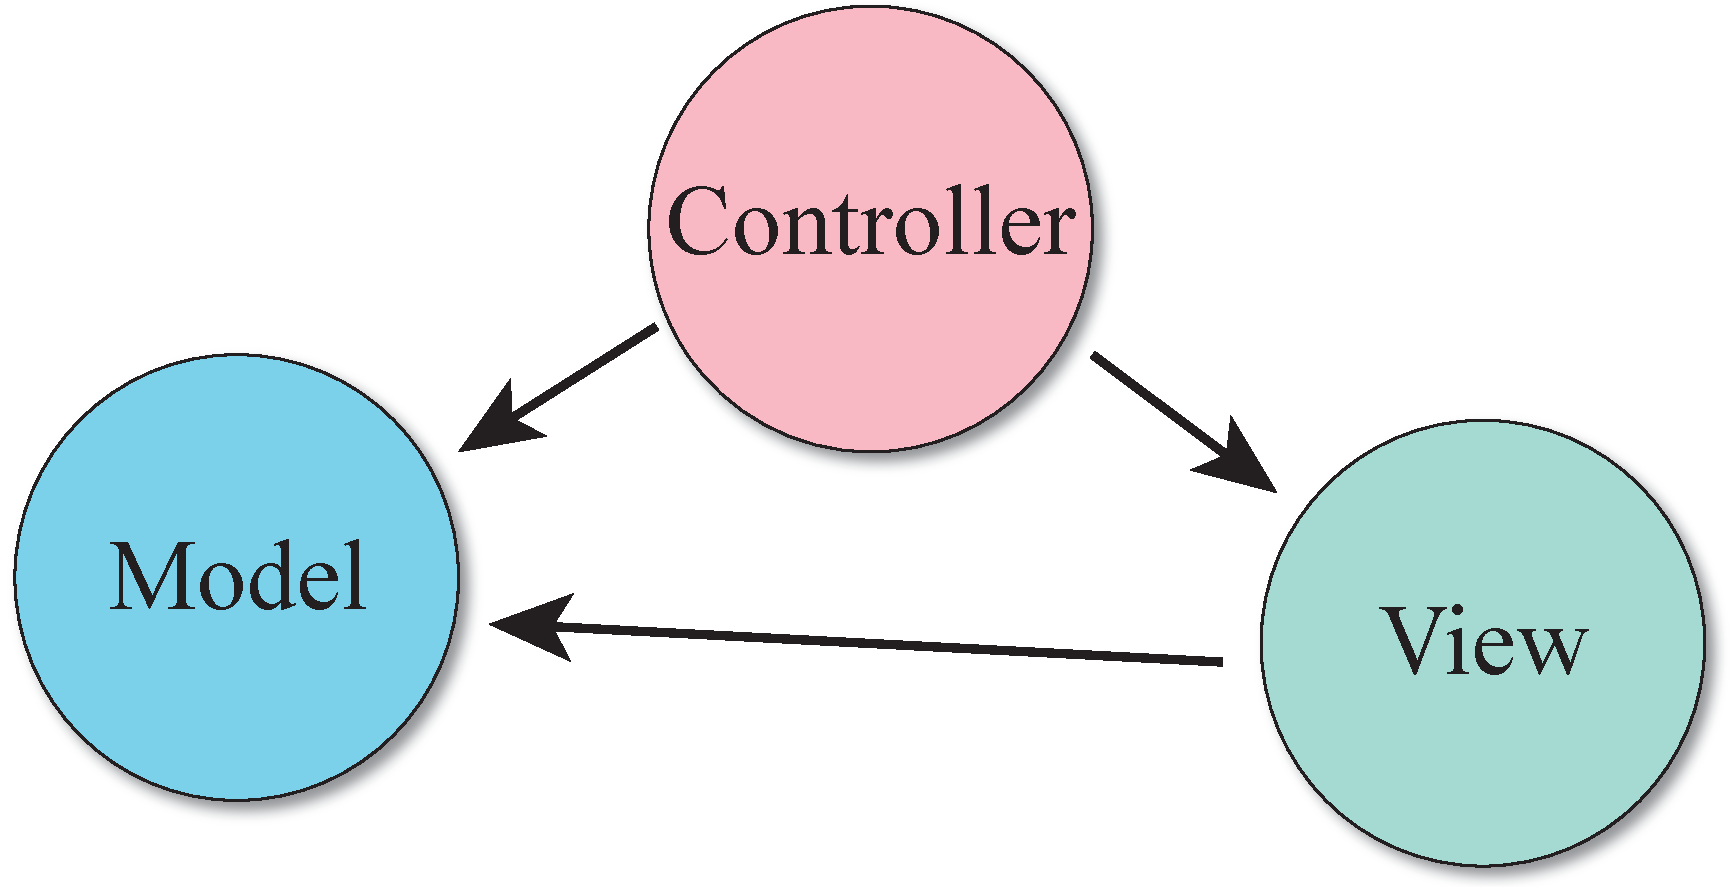
\includegraphics[width=10cm]{fig/mvc}
	\caption{Direkte Assoziationen zwischen Model, View und Controller}
\end{figure}

\paragraph{Model:}
Verantwortlich für alles, was die Daten eines bestimmten Models angeht. In der Anwendung ist dieser Bereich für Interaktionen, Gültigkeit und Auswertung verantwortlich und repräsentiert hier zum Beispiel eine Veranstaltung, ein Benutzer, Statistiken oder Koordinaten der Benutzer.

\paragraph{View:}
Generiert das Aussehen einer bestimmten Seite. Hier wird vorwiegend mit gängigen Webformaten, wie HTML, PHP und JavaScript gearbeitet. Ein View kann auf die Daten zugreifen, die ihm der Controller liefert und diese dann anschaulich darstellen. Dadurch muss sich ein View nicht darum kümmern, woher er seine Informationen zusammensuchen muss, sondern bekommt garantiert, dass diese vom Controller bereit gestellt werden. Auf diese Weise können verschiedene Views für verschiedene Geräte erstellt werden und erlauben einfach eine mobile Seite zu generieren.

\paragraph{Controller:}
Hier findet die gesamte Logik und Aufbereitung der Daten statt, die später dem Benutzer im View angezeigt werden sollen. Sämtliche Datenbankabfragen, Berechnungen oder Ähnliches werden hier durchgeführt und dem Model / View bereitgestellt. Für jedes Objekt existiert ein eigener Controller. Diese werden \emph{EventsController}, \emph{UsersController} etc. genannt.\\
In diesem Framework ist jede Funktion direkt mit den Views verknüpft, das heißt definiert man im EventsController eine Funktion namens \emph{index()}, so stellt dies eine Seite der Webanwendung dar, die mit \emph{http://localhost/Events/index} aufgerufen werden kann und den entsprechenden View in \emph{/View/Events/index.ctp} erwartet.\par

Die Vorteile bei diesem Entwurfsmuster liegen auf der Hand: Es muss nur einmal ein Objekt im Model definiert werden. Im Controller wird die komplette Logik verarbeitet und damit kann man mit entsprechenden Views für verschiedene Ansichten (z.B. eine mobile Anwendung der App) einfach auf die Daten des Controllers zugreifen. Der Code kann dadurch kompakter gehalten werden und muss nur im Controller angepasst werden, um auf allen Ansichten der Seite die Daten aktualisieren zu können.

%%%%%%%%%%%%%%%%%%%%%%%%%%%%%%%%%%%%%%%%%%%%%%%%%%%%%%%%%%%%%%%%%%%%%%%%%%%%%%%%%%%%%%%%%%%%%%%%%%%%%%%%%%%%%%%%%%%%%%%%%%%%%%

\section{Datenbanken}
Um alle Daten schnell und einfach verarbeiten zu können, ist eine Datenbank nötig. Da es sich hier um eine Webanwendung handelt, bietet sich eine SQL Datenbank an, weil diese in der Regel zum Komplettpaket eines Webservers gehört.\par

Als einfachste Möglichkeit wird hier eine MySQL Datenbank verwendet, da sich diese Open-Source-Datenbank in der Praxis durchgesetzt hat. Außerdem ist ein relationales Datenbanksystem die richtige Wahl für diesen Verwendungszweck, da mit einem einheitlichen Schema in die Datenbank geschrieben und auch daraus gelesen werden soll.\\
Folgende Tabellen wurden daher angelegt:\par

\paragraph{users:}
Ein Benutzer besteht aus einer eindeutigen Identifizierungsnummer (\emph{ID}), einem Benutzernamen, einem Passwort und einer zugewiesenen Rolle (z.B. Administrator, Benutzer usw.). Dazu werden von der App automatisch zwei Zeitstempel mit Erstellungs- und letztem Änderungsdatum sowie einem Feld hinzugefügt, welches prüft, ob der Benutzer sich im System der Webanwendung einloggen kann und damit Daten einsehen kann.

\paragraph{events:}
Jede erzeugte Veranstaltung wird hier hinein gespeichert. Verpflichtende Felder sind ein Titel und eine Beschreibung. Dazu wird von der App eine eindeutige ID zugewiesen und die Benutzer-ID des Benutzers hinzugefügt, welcher diese Veranstaltung erstellt. Dazu noch zwei Zeitstempel: Erstellungsdatum und Zeitpunkt der letzten Änderung.\par

Dies sind die beiden grundlegenden Tabellen, die für diese Anwendung nötig sind. Jedoch besteht noch keine Verknüpfung untereinander, abgesehen von der Benutzer-ID in der \emph{events}-Tabelle.

\subsection{Verknüpfung von Benutzer und Veranstaltung}
Um einer Veranstaltung beliebig viele Benutzer zuordnen zu können, wurde die Tabelle \emph{events\_users} erstellt. Diese beinhaltet nur die Fremdschlüssel ID aus den \emph{events} und \emph{users} Tabellen.

\begin{figure}[!ht]
	\centering
	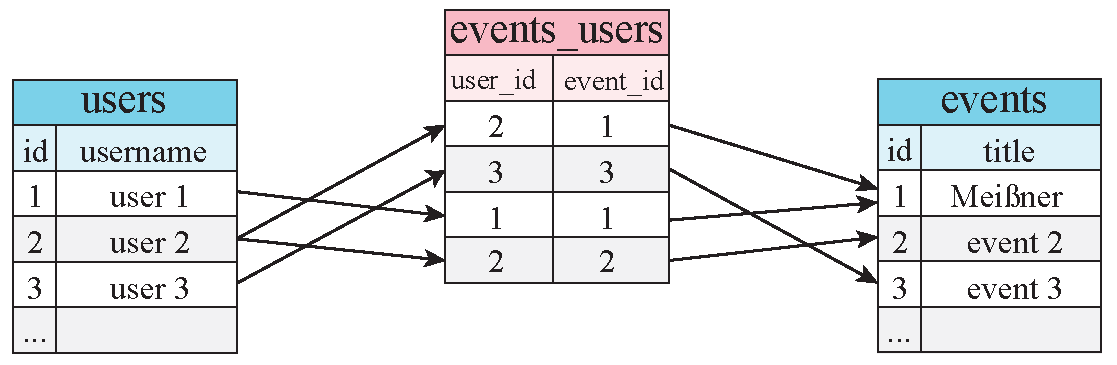
\includegraphics[width=15cm]{fig/events_users}
	\caption[Zuweisung eines Benutzers zu einer Veranstaltung]{Zuweisung eines Benutzers zu einer Veranstaltung (vereinfacht)}
\end{figure}

Diese \emph{Many-to-many}-Verknüpfung (in cakePHP auch \emph{hasAndBelongsToMany, HABTM} genannt) kann der EventsController mit einer einzigen SQL-Abfrage erfragen und erhält damit alle dem Event zugeordneten Benutzer. Diese Daten können dann in einer Variable gespeichert und dem View bereitgestellt werden.

\subsection{Veranstaltungsspezifische Eigenschaften}
Die ersten Schritte zu einer Webanwendung, die Veranstaltungen und Benutzer verwalten kann, sind nun erledigt. Bisher ist es allerdings nicht möglich in Veranstaltungen Felder zu definieren, die für eben jene Veranstaltung von Bedeutung sind. Das können im konkreten Fall Felder sein wie \glqq Art des Transportmittels\grqq{}, \glqq Wird ein Parkplatz benötigt?\grqq{}, \glqq Welcher Holzstangenbedarf besteht?\grqq{} oder Ähnliches.\par

\paragraph{Key-Value-Store} In einem Key-Value-Store wird die Datenbank mit den Werten (\emph{values}) über die Schlüssel (\emph{keys}) indexiert. Der Vorteil ist, dass vorher nicht bekannt sein muss, welche Werte in die Datenbank eingetragen werden sollen. In der Meißner App wurde diese Methode implementiert, um eventspezifisch ein beliebiges Feld zu definieren, welches Werte als Strings annimmt.\\
So ist gewährleistet, dass die Benutzer dieser Anwendung die größtmögliche Freiheit besitzen, was die Inhalte der Veranstaltungen angeht. Jede kann individuell angelegt und personalisiert werden, sodass sie den gewünschten Anforderungen genügt.\\
Als Format für die Values wurden hier ausschließlich Strings gewählt, um den gesamten Vorgang zur Erstellung von speziellen Feldern möglichst gering zu halten. In der späteren statistischen Auswertung ist die Beschränkung des Feldes auf Strings irrelelevant, da sich diese sehr einfach beispielsweise mit PHP verwerten lassen.\par

\paragraph{Implementierung}
Für die Implementierung sind zwei weitere Tabellen notwendig: 

\begin{enumerate} 
	\item \emph{event\_columns}: Dient als Maske, um Feldnamen und -typen zu definieren. Kann zudem innerhalb einer speziellen Veranstaltung genutzt werden, um diese Felder den zugeordneten Benutzern verfügbar zu machen.
	\item \emph{event\_properties}: Nachdem vom Controller die Feldnamen des Events abgefragt wurden, werden diese in einer Variable gespeichert und dem View übergeben. Im View wird dann ein Formular generiert, welches die Feldnamen aus \emph{event\_columns} anzeigt und die Möglichkeit gibt, Werte einzutragen. Diese Werte werden dann über den Controller in \emph{event\_properties} gespeichert.
\end{enumerate}

Mit den Tabellen steht nun die Datenstruktur zur Verfügung, die es ermöglicht verantstaltungsspezifische Eigenschaften zu erstellen und die so erzeugten Feldern mit den entsprechenden Werten der Teilnehmer dieser Veranstaltung zu befüllen.

\begin{figure}[!ht]
	\centering
	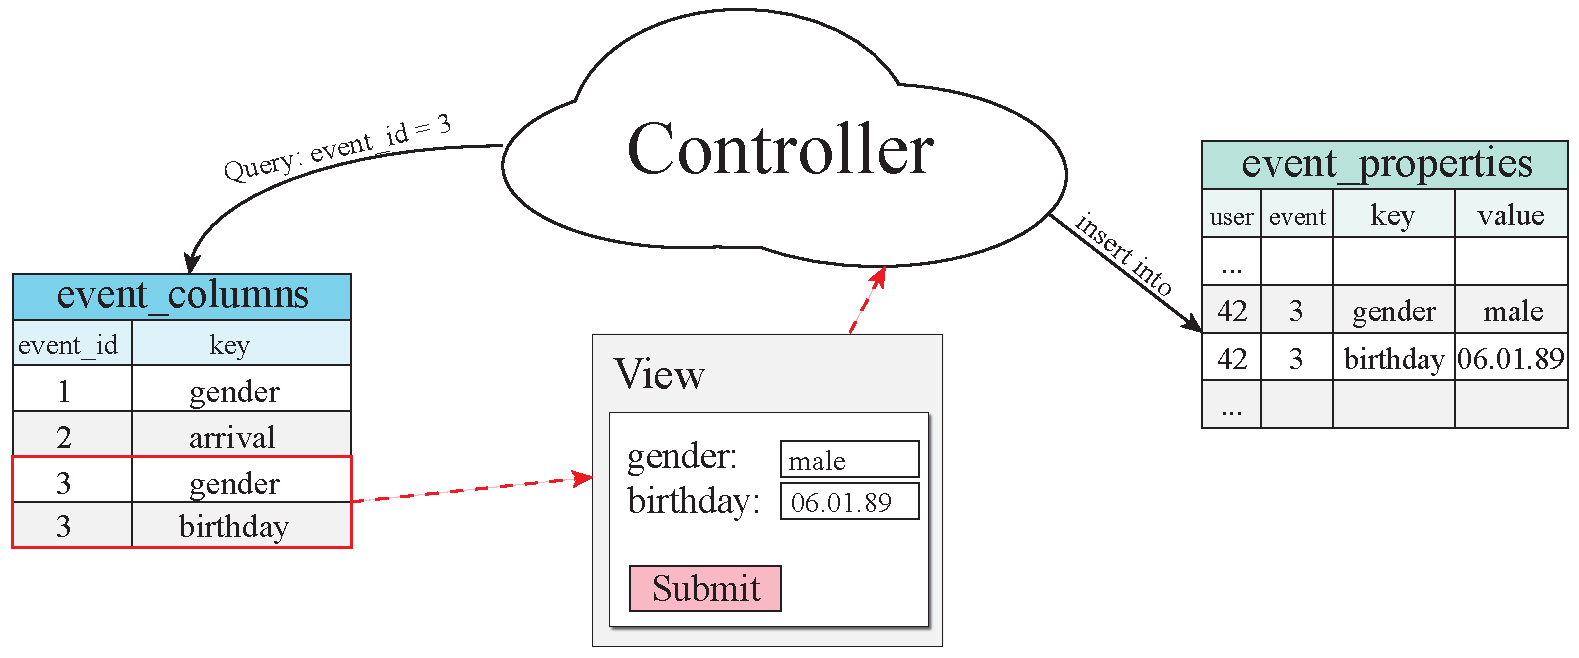
\includegraphics[width=15cm]{fig/event_properties}
	\caption[Speichern von spez. Feldern in die Datenbank]{Controller erfragt Felder aus event\_columns, stellt sie dem View zur Verfügung, speichert danach die Werte in event\_properties}
\end{figure}

Obige Abbildung zeigt kurz das Zusammenspiel von Controller und View: Datenbankzugriffe werden über den View an den Controller gerichtet und dort ausgeführt. So können Daten abgefragt oder neue Daten geschrieben werden.

\section{Views entwickeln}
Eine spannende Herausforderung ist es nun mit modernen Webtechnologien und möglichst geringem Aufwand direkt eine mobile Seite der Anwendung zu erstellen, welche für Smartphone und Tablets optimiert ist. Schließlich soll und muss diese Web-App auch auf dem zugehörigen Platz mobil genutzt werden können.\par

Dabei gibt es mehrere Ansätze, wobei für diese Arbeit das sogenannte \emph{Responsive Webdesign} (deutsch: bedarfsgesteuertes Webdesign) für die mobile Version der Anwendung benutzt wird.

\subsection{Responsive Webdesign mit jQuery Mobile}
Hauptaugenmerk wird hier meistens auf die Auflösung des Endgeräts gelegt: Handelt es sich hierbei um ein günstiges Smartphone mit schlechtem Display, um ein Google Nexus 10 mit 2560x1600 Pixeln oder um einen SmartTV mit FullHD?\\
Diese Frage ist entscheidend, denn sie bestimmt wie viele und wie groß bestimmte Objekte im Sichtbereich des Geräts sein können, sodass der Benutzer nicht von der schlechten Bedienung genervt ist, sondern weiterhin die Informationen aus der App holen möchte. Beim Responsive Webdesign werden über \emph{Media Queries} (Abfrage der Eigenschaften des Geräts, Beispiel: Auflösung, Orientierung des Endgeräts usw.) Informationen des Endgeräts eingeholt und darauf abgestimmte Stylesheets geladen.\par

Um aber eine Webanwendung zu entwickeln, die aussieht und sich \glqq anfühlt\grqq{} wie eine echte App wurde in dieser Arbeit das Framework \emph{jQuery Mobile} verwendet, welches auch auf Responsive Webdesign setzt und dabei viele Steuerelemente zur Verfügung stellt, die dem Benutzer schon von nativen Apps her bekannt sind, wie typische Slider, Buttons, Dropdown-Menüs und vielem mehr.\par

So sind lediglich wenige Änderungen am normalen View nötig, um daraus eine mobile Version zu entwickeln, die für die Bedienung mit dem Finger optimiert ist.

\chapter{Echtzeitaktualisierung durch WebSockets}
Das wohl spannendste Thema und die erste große Erweiterung dieser Arbeit ist die Echtzeitaktualisierung im Hintergrund der Web-App. Mehrere Möglichkeiten sind dafür gegeben, wobei einige besser geeignet sind als andere.

\section{Vor HTML5: Benutzung von Polling}
Für den Datenverkehr von Internetseiten wird HTTP benutzt, welches die wechselseitige Datenübermittlung \emph{Halbduplex} verwendet. So erfolgt der Datenverkehr nur in eine Richtung zur gleichen Zeit: der Client schickt eine Anfrage an den Server und dieser übermittelt danach die Antwort \cite[S. 5]{ws}. Das hat wiederum zur Folge, dass es relativ ineffizient ist, da man mit jeder Anfrage stets die Antwort des Servers abwarten muss.\par

\begin{figure}[!ht]
	\centering
	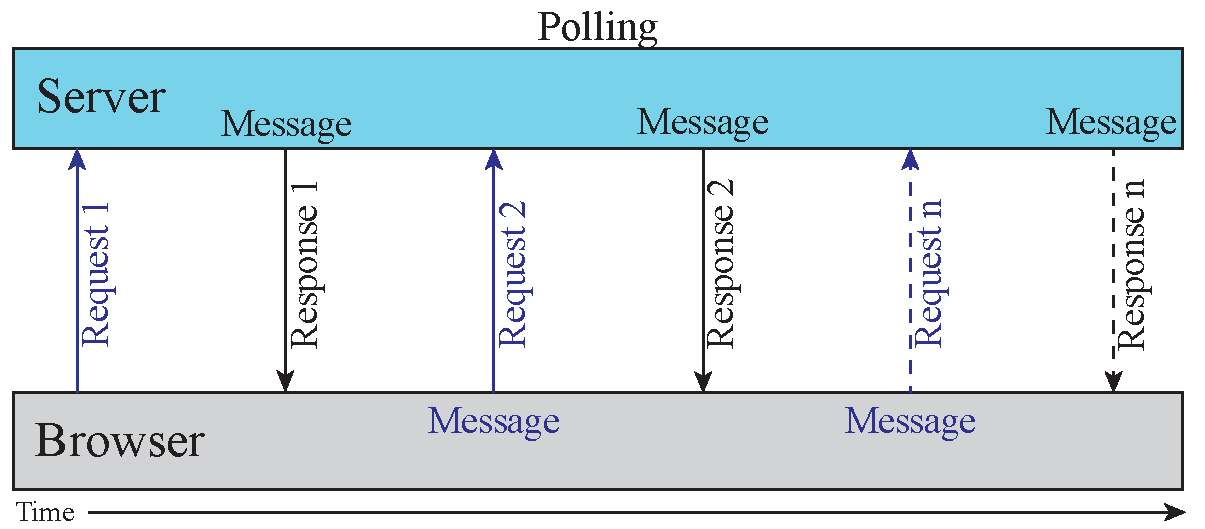
\includegraphics[width=15cm]{fig/polling}
	\caption{Datenaustausch mittels HTTP Request / Response beim Polling {\cite[S. 7]{ws}}}
\end{figure}

Vor diesem technischen Hintergrund wurde Polling entwickelt, bei dem in einem zeitlich bekannten Intervall eine Anfrage an den Server geschickt wird mit der Bitte um Aktualisierung. Diese Technik ist sehr attraktiv, wenn die zeitlichen Abstände der Aktualisierung der Daten bekannt ist, allerdings sind Echtzeitdaten schlecht vorhersehbar. Dadurch ist Polling nicht die richtige Wahl für dieses Projekt, weil es auf eine wirkliche Echtzeitaktualisierung ankommt.\par

\section{Einführung in WebSockets}
Mit der HTML5-Spezifikation wurden \emph{WebSockets}, ein auf TCP basierendes Netzwerkprotokoll, eingeführt, welches eine Vollduplex, bidirektionale, Single-Socket Verbindung ermöglicht \cite[S. 7]{ws}. Eine Anfrage öffnet die Verbindung zum WebSocket Server und kann beliebig lange offen gehalten werden, wobei zu jeder Zeit Daten zwischen Client und Server ausgetauscht werden. Der erste Handshake erfolgt über HTTP/1.1 und ähnelt dem zum Aufruf einer Homepage.
\\
\begin{lstlisting}[captionpos=b, caption=HTTP Request vom Client {\cite[S. 6]{rfc6455:handshake}}]
  GET / HTTP/1.1
  Host: server.example.com
  Origin: http://www.example.com
  Sec-WebSocket-Key: 7+C600xYyb0v2zmJ69RQsw==
  Sec-WebSocket-Version: 13
  Upgrade: websocket
\end{lstlisting}

Mit \emph{Upgrade: websocket} wird signalisiert, dass der Client eine WebSocket-Verbindung zum Server aufbauen möchte. Der entsprechende WebSocket Server reagiert darauf mit dem HTTP-Statuscode \emph{101 Switching Protocols}, womit er bestätigt, dass er mit dem Wechsel des Protokolls einverstanden ist.
\\
\begin{lstlisting}[captionpos=b, caption=HTTP Response vom Server {\cite[S. 8]{rfc6455:handshake}}]
  101 Switching Protocols
  Connection: Upgrade
  Sec-WebSocket-Accept: fYoqiH14DgI+5y1EMwM2sOLzOi0=
  Upgrade: WebSocket
\end{lstlisting}

Der kryptische Schlüssel \emph{Sec-WebSocket-Accept} muss vom Server berechnet und zurückgegeben werden und zeigt damit, dass er das WebSocket Protokoll versteht. Ab diesem Zeitpunkt ist der Handshake abgeschlossen und die WebSocket-Verbindung wurde aufgebaut.\par

\begin{figure}[!ht]
	\centering
	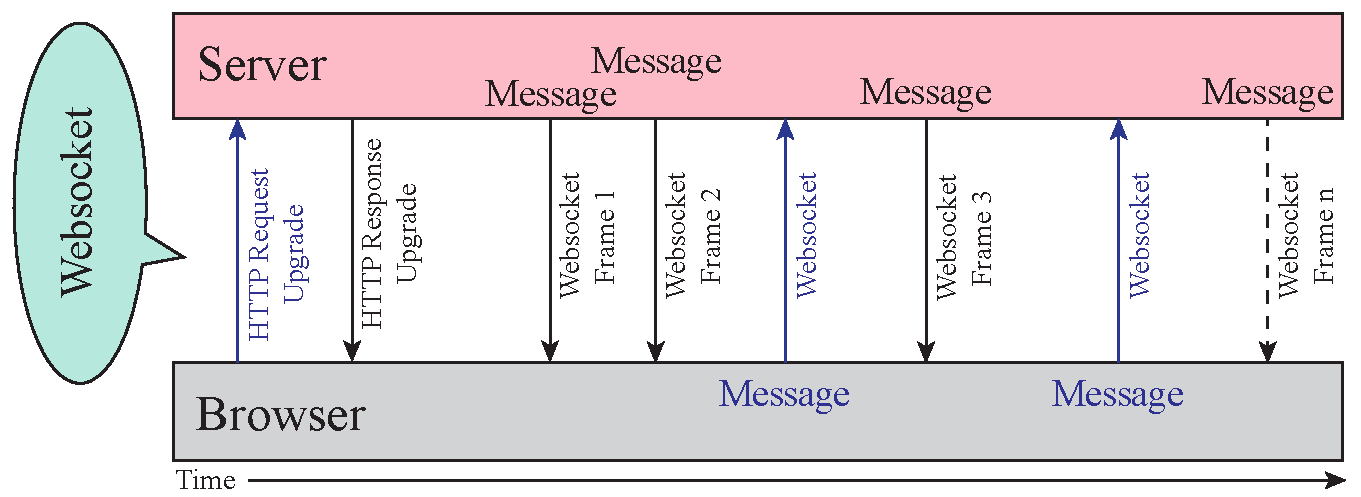
\includegraphics[width=15cm]{fig/websockets}
	\caption{Aufbau einer WebSocket Verbindung. Danach können beliebig Nachrichten in beide Richtungen (gleichzeitig) übermittelt werden}
\end{figure}

Nun kommen die Vorteile von WebSockets zur Geltung: nach erstmaligem Aufbau der Verbindung bleibt diese geöffnet und zu jedem Zeitpunkt können Client und Server die Vollduplex Verbindung nutzen, um Daten miteinander auszutauschen. Das verringert Latenzzeiten (die Pakete werden direkt zugestellt, da der Server auf keinen Request vom Client warten muss), den Traffic (der Overhead ist deutlich geringer, nur ein Handshake zu Beginn erforderlich) und die CPU-Leistung der Server (der Austausch der Daten ist einfacher gestaltet als beim Polling o.Ä.).

\section{Implementierung der Echtzeitaktualisierung}
Im ersten Ansatz dieser Arbeit wurde der WebSocket-Server auf Basis von \emph{node.js} \cite{node.js}, einem serverseitigem JavaScript Framework für Server, implementiert. Das verlief aufgrund der einfachen Handhabung von WebSockets und der guten Unterstützung von HTML5 problemlos. Jedoch wurden zu diesem Zeitpunkt weder verschlüsselte Verbindungen noch Broadcasting unterstützt. Daher war dies ungeeignet, weil sensible Daten, wie die Standorte der Clients, nicht im Klartext verschickt werden sollten.\\
Außerdem ist ein Broadcasting-Funktion notwendig, die den bestehenden Sockets bei Aktualisierung einer Position sofort die neuen Koordinaten übermittelt.\par

Die Implementierung beider Funktionen hätte den Rahmen dieser Arbeit überschritten, weshalb serverseitig das Open Source Modul \emph{socket.io} \cite{socket.io} für node.js verwendet wird, welches sämtliche benötigten Dienste bereitstellt und dabei noch einen Fallback zur Verfügung stellt, wodurch auch älteren Browsern ohne HTML5 Unterstützung eine websocketähnliche Verbindung ermöglicht wird.\par

Clientseitig wurde eine Routine in JavaScript entwickelt, welche im Hintergrund der Web-App ausgeführt wird. Dieses Skript verbindet sich mit dem WebSocket Server, schickt initial die aktuellen Koordinaten (unabhängig davon, welcher View gerade angezeigt wird) und wartet auf eingehende Nachrichten oder auf eine Änderung der eigenen Position. Bewegt sich der Client werden automatisch die Koordinaten GoogleMaps-kompatibel in Form von Latitude und Longitude an den WebSocket Server übermittelt.\\
Erhält der Server so eine Nachricht, aktualisiert er seine Datenbank von Standorten der Clients und schickt per Broadcast eine Nachricht an alle verbundenen Clients. So erhalten die Endgeräte in Echtzeit eine Aktualisierung aller Positionen.\par

Beendet ein Client die Verbindung oder erhält der Server keine Aktualisierungen mehr, so wird sein letzter Standort noch 15 Minuten gespeichert und dann auf allen Endgeräten gelöscht. Zu keiner Zeit werden Daten protokolliert oder länger als nötig gespeichert.\par

\paragraph{Schwierigkeit beim Wechseln oder Neuladen eines Views.}
Ein Problem, welches bei der Nutzung von WebSockets (kurz: WS) auftrat, war der Übergang zwischen den einzelnen Seiten: Wird eine Seite gewechselt, so wird die WebSocket Verbindung geschlossen, die nächste Seite per HTTP Request angefordert und eine neue Verbindung zum WS Server aufgebaut. Also wird mit jedem Wechsel ein neuer Socket erstellt, den der Server neu zu den bestehenden Daten des Clients referenzieren muss.\\
Damit ist nun durch neue Assoziationen von Referenzen ein Wechsel zwischen den Views möglich, ohne dabei Werte wie Positionen des Clients zu verlieren, möglich.

\paragraph{Entwicklung eines eigenen Protokolls zur Kommunikation über WebSockets.}
Um bestimmte Funktionen auf dem Server anzusprechen, wurde ein einfaches Protokoll entwickelt, welches angibt, um welchen Inhalt es sich bei der Nachricht handelt. So haben alle Nachrichten, die zwischen Client und Server ausgetauscht werden, ein bestimmtes Format und ein Feld \emph{type}, welches aktuell folgende Werte annehmen kann:

\begin{itemize}
	\item[] \emph{location:} enthält Latitude und Longitude des Clients
	\item[] \emph{syn:} enthält eine Signatur, die überprüft wird
	\item[] \emph{subscribe:} abonniert bestimmte Events, dazu später mehr
	\item[] \emph{publish:} signalisiert eine Änderung an der Datenbank
	\item[] \emph{message:} eine neue Chat Nachricht hat den Server erreicht und wird per Broadcast an die Clients verschickt
	\item[] \emph{history:} Anfrage eines Clients nach der aktuellen Historie des Chats
\end{itemize}

Der socket.io Server wertet diese Fälle über ein \emph{Switch-Case-Statement} aus und ruft entsprechende Methoden zur weiteren Verarbeitung auf.

\section{Authentifizierung eines Clients beim WebSocket Server}
In der anfänglichen Implementierung der Skripte für die Kommunikation zwischen Client und Server war es noch möglich die Positionsdaten von Benutzern abzufangen, indem man sich simpel für diese beim WS Server ausgegeben hat. Wenn der Server eine Nachricht bekommen hat mit Inhalt \emph{Ich bin \glqq BenutzerXY\grqq{}}, so wurde diese Verbindung in die Liste der verbundenen Sockets des Accounts eingetragen und so konnte der \glqq Angreifer\grqq{} alle Standorte der Clients beim nächsten Broadcast empfangen.\par

Über das Public-Key-Verschlüsselungsverfahren wurde dann eine serverseitige Methode implementiert, die bei der ersten Initialisierung der Meißner-Webanwendung mit \emph{openssl} je einen öffentlichen und privaten RSA Schlüssel erstellt. Mit diesem privaten Schlüssel wird eine Signatur der Nachricht des Typs \emph{syn} erstellt, an die Nachricht angehangen und dem WebSocket Server zugeschickt.\\
Socket.io erkennt ein \emph{syn} und die Signatur, öffnet den öffentlichen Schlüssel der Webanwendung und überprüft so die Signatur. Sofern diese gültig ist, wird der Client, der die Nachricht übermittelt hat, in die Liste der gültigen Clients eingefügt.\par

Dadurch ist garantiert, dass die Signatur der Web-App wirklich nur von dieser Anwendung stammt und es sich damit um einen normalen Benutzer handelt. Andernfalls wird die Verbindung mit der Fehlermeldung \emph{unauthorized} abgewiesen.\par

Alle weiteren Typen von Nachrichten können nun durch eine einfache \emph{default: deny} Regel alle einkommenden Nachrichten verwerfen, die von Verbindungen stammen, welche vorher keine Authentifizierung beim Server vollzogen haben. Das spart Rechenleistung, denn es muss nur ein kurzer Vergleich der Objektreferenz erledigt werden.\par


\section{Entwurfsmuster: Publish / Subscribe}
Da die Meißner App nun über eine Echtzeitaktualisierung verfügt, wird diese auch genutzt, um das \emph{Publish / Subscribe} Muster anzuwenden. Hierbei können Clients bestimmte Events abonnieren (= subscribe). Das funktioniert ebenfalls im Hintergrund und wird nach dem Einloggen des Benutzers an den WebSocket Server übermittelt über eine \emph{subscribe}-Nachricht. Standardmäßig werden alle Veranstaltungen abonniert, die der jeweilige Benutzer erstellt hat.\\
Dazu wird noch die Möglichkeit implementiert per Klick auf einen Button eine bestimmte Sache zusätzlich zu abonnieren.\par

Gab es eine Änderung an einer Veranstaltung, so meldet sich die Web-App beim WebSocket Server mit einer \emph{publish}-Nachricht. Dieser schaut dann in seiner Liste der authentifizierten Clients nach, welcher die Veranstaltung abonniert hat und schickt an alle verbundenen Endgeräte des Benutzers eine Mitteilung, dass seine Veranstaltung bearbeitet wurde.\par

Bei diesem Entwurfsmuster wissen weder Publisher noch Subscriber voneinander und es läuft vollkommen unabhängig, asynchron miteinander. Sie müssen auch nichts voneinander wissen, da sämtlicher Datenaustausch über den socket.io Server läuft \cite{autobahn.js:pubsub}.

\paragraph{Probleme dieser Implementierung.}
Im ersten Entwurf der Technik in dieser Arbeit wurden alle Nachrichten, die über WebSockets verschickt wurden, über die Clients selbst geregelt. Das hatte den Grund, dass socket.io und die Entwicklungsumgebung node.js vollständig in JavaScript entwickelt wurden und daher die Kompatibilität zu dieser Skriptsprache komplett gegeben war. Das jeweilige Endgerät muss dafür nur das socket.io Modul vom Server laden und kann dann direkt Nachrichten verschicken.\\
Die Webanwendung verwendet hauptsächlich PHP5 und die Views/Layouts HTML5 - für diese Sprachen stellt socket.io aber keine Bibliothek zur Verfügung, um sich mit dem WS Server zu verbinden. Es hat auch zur Folge, dass keine WebSockets verschickt werden können.\par

Dass eine derartige Implementierung nicht ideal ist, ist sofort ersichtlich. Man stelle sich folgendes Szenario vor: ein Benutzer ist mit einem Endgerät eingeloggt, welches die Nutzung von JavaScript unterbindet. Er verändert nun eine Veranstaltung, kann aufgrund des abgeschaltetem JavaScript keine \emph{publish}-Nachricht verschicken, weshalb die Benutzer, die diese Veranstaltung abonniert haben, keine Aktualisierungsmeldung erhalten. Leider würde damit das Publish / Subscribe-Modul nicht zuverlässig funktionieren.

\paragraph{Verbesserung des Moduls.}
Eine bessere Lösung ist es, wenn die Meißner App selbst publishen könnte. Deshalb wurden auf Basis von Elephant.io \cite{elephant.io}, einer Open Source Bibliothek, welche die Verbindung zu socket.io über PHP5 realisiert, Methoden entwickelt, die die publish-Funktion der Webanwendung übernehmen.\\
Der EventsController hat nun noch die zusätzliche Aufgabe bei jedem Datenbankzugriff eine Verbindung zum WS Server zu öffnen, eine publish-Nachricht abzuschicken, und dann die Verbindung wieder zu schließen.\par

Dadurch funktioniert Publish/Subscribe auch mit Endgeräten, die JavaScript verbieten und die Clients, die Nachrichten erhalten möchten, bekommen diese nun ungehindert zugestellt.

\section{Umgebungsbedingte Einschränkungen}
Bei diesem Projekt handelt es sich um eine Webanwendung, die aufgrund von Sicherheitsvorkehrungen einigen Einschränkungen unterliegt. So erlauben die mobilen Browser keine Geopositionierung durch den Browser, wenn dieser minimiert ist oder das Smartphone / Tablet nicht aktiv genutzt wird. Das bedeutet, dass die Meißner App geöffnet sein muss, damit alle Funktionen genutzt und aktualisiert werden können.\par

Das ist für die Lokalisierung problematisch, da so die Position des Clients nicht aktuell bleibt. Diese Sicherheitsmaßnahmen sind jedoch sehr sinnvoll, denn es wäre sehr bedenklich könnte eine Homepage im Hintergrund stetig die Position des Besuchers überwachen. Allerdings genügt es, wenn die Webanwendung in einem Tab geöffnet ist, welcher nicht aktiv sein muss, um die Position des Endgeräts zu erfahren.

\chapter{Erweiterte Funktionen}
In diesem Kapitel werden nun weitere Funktionen beschrieben, die über die Grundausstattung der Web-App und die WebSockets hinausgehen, um diese zu erweitern und produktiver zu gestalten. 

\section{Entwurfsmuster: Publish / Subscribe}
Mit Publish / Subscribe (deutsch: veröffentlichen / abonnieren) wird ein Muster beschrieben, mit dem ein Client eine Benachrichtigung erhält, sofern ein Ereignis verändert wurde, welches von ihm abonniert wurde. Bei diesem Entwurfsmuster wissen weder Publisher noch Subscriber voneinander und es läuft vollkommen unabhängig, asynchron miteinander. Sie müssen auch nichts voneinander wissen, da sämtlicher Datenaustausch über den socket.io Server läuft \cite{autobahn.js:pubsub}.\par

Konkret können in dieser Anwendung Veranstaltungen abonniert werden. Das geschieht automatisch über die Webanwendung selbst, welche dem WebSocket Server mit Einloggen des Benutzers eine subscribe Nachricht schickt. Ausgewählt werden die Events, die der Benutzer selbst erstellt hat. 

Gab es eine Änderung an einer Veranstaltung, so meldet sich die Web-App beim WebSocket Server mit einer \emph{publish}-Nachricht. Dieser schaut dann in seiner Liste der authentifizierten Clients nach, welcher die Veranstaltung abonniert hat und schickt an alle verbundenen Endgeräte eine Mitteilung, dass die Veranstaltung bearbeitet wurde.\par

\paragraph{Implementierung}
Im ersten Entwurf der Technik in dieser Arbeit wurden alle Nachrichten, die über WebSockets verschickt wurden, über die Clients selbst versendet, da die Kommunikation nur über JavaScript nativ unterstützt wird. Daher wurden auf Basis von Elephant.io \cite{elephant.io}, einer Open Source Bibliothek, welche die Verbindung zu socket.io über PHP5 realisiert, Methoden entwickelt, die die publish-Funktion der Webanwendung übernehmen.\\
Der EventsController hat nun noch die zusätzliche Aufgabe bei jedem Datenbankzugriff eine Verbindung zum WS Server zu öffnen, eine publish-Nachricht abzuschicken, und dann die Verbindung wieder zu schließen.\\
Dadurch funktioniert Publish/Subscribe auch mit Endgeräten, die JavaScript verbieten. Die Clients, die Nachrichten erhalten möchten, bekommen diese nun ungehindert zugestellt.\par

\begin{figure}[!ht]
	\centering
	
\includegraphics[width=15cm]{fig/noty_android}
	\caption{publish-Benachrichtigung am unteren Bildschirmrand mit Android}
\end{figure}

So ist es nun möglich über WebSockets eine Benachrichtigung an die Abonnenten zu schicken. Dadurch wird man aktiv informiert, wenn Änderungen an den Veranstaltungen vorgenommen werden. 

\section{Lokalisierung von Clients}
Mit HTML5 wurde die \emph{navigator.geolocation} Klasse in die JavaScript API eingebaut. Diese Klasse ermöglicht es einer Webanwendung die Position des Anwenders zu erhalten - aber nur, wenn der Anwender zustimmt. Das geschieht mittels in der Umgebung befindlichen W-Lan Netzwerke, der eigenen IP und wird dann mit einem Google Service abgeglichen. Verfügt das Gerät über GPS, so werden diese Daten auch berücksichtigt und ermöglichen eine genauere Ortung \cite[1. Absatz]{html5:geolocations}.

\paragraph{Koordinieren von Helfern}
Um die eingetragenen Helfer in dieser Webanwendung besser koordinieren zu können, wurde daher ein Skript implementiert, welches im Hintergrund der Web-App läuft und die aktuelle Position des Endgeräts über eine SSL verschlüsselte Verbindung an den Server übermittelt. Unter der Voraussetzung, dass der Client diesem Vorgang zustimmt sind dem Server damit die Positionen der eingeloggten Benutzer bekannt. Diese Positionsdaten können dann von der Anwendung ausgewertet und in einer Karte von Google Maps visualisiert werden.\par

Jeder Client kann auf diese Weise die Positionen der anderen Helfer sehen. Der Vorteil liegt klar auf der Hand: eine zentral eingerichtete Verwaltung kann mit einem Blick sehen, wer sich an welcher Stelle auf dem Gelände befindet. So können Wege optimiert und gezielt Aufgaben an sogenannte Springer verteilt werden, da ortsnahe Helfer die entsprechenden Aufgaben übernehmen können. Die kurzen Wege sorgen dann dafür, dass eine höhere Nutzung der Ressourcen (hier: die Helfer) möglich ist.\par

\paragraph{Anforderungen}
Eine wichtige Anforderung an diese Funktion ist, dass die Daten schnell ausgetauscht werden. Wenn zwischen den Updates der Geolocations zu viel Zeit vergeht, ist die Position nicht mehr aktuell und damit nicht mehr relevant. Deswegen findet der Austausch von Longitude und Latitude auch über WebSockets statt.

\paragraph{Speichern der Positionsdaten}
Beendet ein Client die Verbindung oder erhält der Server keine Aktualisierungen mehr, so wird sein letzter Standort noch 15 Minuten gespeichert und dann auf allen Endgeräten gelöscht. Zu keiner Zeit werden Daten protokolliert oder länger als nötig aufbewahrt.

\subsection{Umgebungsbedingte Einschränkungen}
Bei diesem Projekt handelt es sich um eine Webanwendung, die aufgrund von Sicherheitsvorkehrungen einigen Einschränkungen unterliegt. So erlauben die mobilen Betriebssysteme keine Geopositionierung durch den Browser, wenn dieser minimiert ist oder das Smartphone / Tablet nicht aktiv genutzt wird. Das bedeutet, dass die Meißner App geöffnet sein muss, damit alle Funktionen genutzt und aktualisiert werden können.\par

Das ist für die Lokalisierung problematisch, da so die Position des Clients nicht aktuell bleibt. Diese Sicherheitsmaßnahmen sind jedoch sehr sinnvoll, denn es wäre sehr bedenklich könnte eine Homepage im Hintergrund stetig die Position des Besuchers überwachen. Allerdings genügt es, wenn die Webanwendung in einem Tab geöffnet ist, welcher nicht aktiv sein muss, um die Position des Endgeräts zu erfahren.

\section{Paketierung für App-Stores}
Auch bei Web-Apps besteht die Möglichkeit diese in den gängigen App-Stores wie dem von Apple oder Googles Play Store anzubieten. Dafür gibt es einige Frameworks, welche die eigentliche Webanwendung in eine Browserumgebung verpacken und diese dann wie eine native App aussehen lassen.\par
Für diese Arbeit wurde bewusst nicht darauf eingegangen und auch keine Paketierung für die Stores eingeplant. Das gesamte Projekt soll sehr dynamisch sein und ohne Grenzen der Stores für alle Geräte zur freien Verfügung stehen. Und eine Webseite aufrufen ist da die einfachste Möglichkeit die Anwendung zu nutzen.

\paragraph{Vorteile}
So können Änderungen an der Meißner App vorgenommen werden ohne, dass man kompliziert über die Stores die App neu verteilen muss. Außerdem ist absolut keine Installation notwendig, da sie wie eine normale Homepage geladen wird. Der Benutzer ist zwar nicht zwangsläufig gewohnt Apps über einen anderen Weg als den bekannten Store zu beziehen, aber da die Web-App genau so einfach geöffnet wird wie der Aufruf einer Homepage, kann man davon absehen.

\subsection{Add to Homescreen}
Einzig für aktuelle iOS Geräte, wie dem iPhone oder iPad, gibt es die Möglichkeit ein appähnliches Erlebnis zu bekommen: Durch die Funktion \emph{Add to Homescreen} ist die Webanwendung über ein gewohntes Icon zu erreichen. Durch eine einfache Ergänzung im Header der mobilen HTML Seite wird so eine appähnliche Installation ermöglicht.
\\
\begin{lstlisting}[captionpos=b, caption=Ergänzung im Header der mobilen Seite]
  <meta name="apple-mobile-web-app-capable" content="yes">
  <meta name="apple-mobile-web-app-status-bar-style"
  	content="black">
  <link rel="apple-touch-icon" href="img/icon.png">
\end{lstlisting}
Mit diesen drei Zeilen wird zuerst die Option \emph{Add to Homescreen} erlaubt, dann die Statusleiste schwarz gefärbt und der Pfad zum Icon angegeben, welches dann auf dem Homescreen erscheinen soll.\par

Das stellt einfache Möglichkeit dar eine Web-App zu installieren, allerdings gibt es keine ähnliche Funktion unter anderen Betriebssystemen wie Android o.Ä. Außerdem kennen die wenigsten Benutzer diese Funktion und daher wird sie sicherlich nur sehr wenig genutzt.


\section{PUSH-Benachrichtigungen}
Bei Webanwendungen gibt es noch weitere Einschränkungen. So konnte für diese Arbeit nicht auf die systemeigenen Benachrichtigungsmechanismen zurückgegriffen werden, wie man sie aus nativen Applikationen her kennt. In den aktuellen Versionen aller mobilen Betriebssystemen sind Bereiche für Benachrichtigungen aus den jeweiligen Anwendungen implementiert um dem Benutzer zu signalisieren, dass neue Nachrichten vorliegen. Allerdings darf eine Web-App darauf nicht zugreifen, daher wurden für diese Anwendung eigene Methoden auf Basis von \emph{noty} \cite{noty}, einem jQuery Plugin für Benachrichtigungen, implementiert. Mit dieser Bibliothek wurde eine Benachrichtigungsleiste entwickelt, die am unteren Bildschirmrand Informationen anzeigen kann, wie zum Beispiel die oben angesprochene publish-Benachrichtigung vom WebSocket Server.\par

Auf diese Weise können nun auf allen Plattformen, die JavaScript aktiviert haben, Push-Benachrichtigungen angezeigt werden, wenn relevante Informationen über die WebSockets an das Endgerät gelangen.


\section{Chatfunktion}
Zur Kommunikation der Clients untereinander wurde der Bereich \emph{Chats} hinzugefügt. Denkbar simpel findet der Datenaustausch über WebSockets statt und muss nicht konfiguriert werden. Es muss nur der entsprechende View geöffnet werden und die Webanwendung verbindet sich automatisch mit dem socket.io Server, holt sich die Historie vom Server und zeigt sie an. Ein einfaches Eingabeformular ermöglicht dann die Kommunikation mit allen eingeloggten Benutzern.


\section{Statistiken}
Da eine Auswertung der eingegebenen Daten für Veranstaltungen unabdinglich ist, wurde ein weiterer Controller implementiert, welcher sämtliche speziellen Felder der Events aus der Datenbank abfragt und diesen dann die Werte der einzelnen Benutzer zuweist.\par

Im View wird dann eine grafische Auswertung gestartet, die mit Hilfe von Google Charts ansehnliche Graphen generiert, wo es Sinn ergibt und vergleichbare Werte von den Benutzern hinterlegt wurden. Außerdem gibt es allgemeine Statistiken, die die Veranstaltungen untereinander vergleichen und man so einen schnellen Überblick über die angelegten Events erhält.












%%%%%%%%%%%%%%%%%%%%%%%%%%%%%%%%%%%%%%%%%%%%%%
%%    End of the main document              %%
%%%%%%%%%%%%%%%%%%%%%%%%%%%%%%%%%%%%%%%%%%%%%%

\backmatter

\bibliographystyle{alphadin} %% german output

\bibliography{bachelor}

\printindex

\chapter*{Ehrenwörtliche Erklärung}

Hiermit versichere ich, die vorliegende Bachelorarbeit selbstständig 
verfasst und keine anderen als die angegebenen Quellen und Hilfsmittel
benutzt zu haben.
Alle Stellen, die aus den Quellen entnommen
wurden, sind als solche kenntlich gemacht worden. Diese Arbeit hat in
gleicher oder ähnlicher Form noch keiner Prüfungsbehörde vorgelegen.

\vspace{3cm}

\noindent Düsseldorf, 14.Dezember 2004 \hfill Vorname Nachname


\cleardoublepage

\chapter*{}
\thispagestyle{empty}

\begin{center}
  \vspace{-3cm}
  \fbox{\parbox[c][12cm][c]{12cm}{\centering Hier die H\"ulle\\[1cm]mit der CD/DVD einkleben}}
\end{center}

\vfill

\textbf{Diese CD enthält:}
\begin{itemize}
 \item eine \emph{pdf}-Version der vorliegenden Bachelorarbeit
 \item die \LaTeX- und Grafik-Quelldateien der vorliegenden Bachelorarbeit samt aller verwendeten Skripte
 \item \textbf{[anpassen]} die Quelldateien der im Rahmen der Bachelorarbeit erstellten Software XYZ
 \item \textbf{[anpassen]} den zur Auswertung verwendeten Datensatz
 \item die Websites der verwendeten Internetquellen
\end{itemize}


\end{document}

